% ==============================================================================
% PG - Sophie Dilhon
% Capítulo 2 - Referencial Teórico
% ==============================================================================
\chapter{Referencial Teórico e Tecnologias Utilizadas}
\label{chap-referencial}

% Este capítulo deve apresentar os aspectos relativos ao conteúdo teórico relevante para o trabalho.  Incluirá conhecimento adquirido a partir de livros, artigos, relatórios técnicos, dissertações, teses e outros materiais bibliográficos.  O capítulo deve apresentar, além do referencial teórico, informações sobre as tecnologias utilizadas no trabalho. O capítulo deve ter cerca de 12-15 páginas e deve demonstrar conhecimento básico da literatura técnico-científica sobre o tema abordado no trabalho.


Neste capítulo serão apresentados os referenciais teóricos utilizados para o desenvolvimento
deste trabalho. A Seção \ref{sec-fundteo-engsoft} aborda os conceitos da Engenharia de Software,
em seguida, o método FrameWeb é explicado na Seção \ref{sec-fundteo-frameweb}
e, por fim, as categorias de \textit{frameworks} suportadas pelo método, assim como o \textit{framework}
utilizado neste trabalho são apresentados na Seção \ref{sec-fundteo-framework}.


%%%%%%%%% Início de seção. %%%%%%%%%
\section{Engenharia de Software}
\label{sec-fundteo-engsoft}

A Engenharia de Software é uma área da computação que se preocupa com todo o ciclo de vida do software,
desde a especificação, desenvolvimento e até manutenção de sistemas de software~\cite{sommerville:2011}.
Por meio da aplicação de métodos e ferramentas que possibilitam a construção de sistemas complexos,
tem como objetivo gerar produtos dentro do prazo e com qualidade~\cite{pressman:2011}.
Segundo \citeonline{sommerville:2011}, a Engenharia de Software define quatro atividades
essenciais para todos os processos de software, são elas:


\begin{enumerate}
    \item \textbf{Especificação de software}: são definidas as funcionalidades do 
        sistema, a partir da comunicação cliente e engenheiro;
    \item \textbf{Projeto e implementação de software}: são definidos os modelos 
        arquiteturais e o sistema é implementado;
    \item \textbf{Validação de software}: o software deve ser validado para garantir 
        que os requisitos estejam contemplados;
    \item \textbf{Evolução de software}: são feitas adaptações e evoluções no sistema 
        para atender as necessidades do cliente.
\end{enumerate}

\subsection{Engenharia de Requisitos}
\label{subsec-fundteo-engsoft-engreq}

Como visto anteriormente, é na fase de Especificação de Software que as funcionalidades 
e restrições do sistema são definidas, e é fundamental que os softwares contemplem os
requisitos estabelecidos para garantir um desempenho satisfatório no suporte aos processos 
de negócios. Dessa forma, uma importante tarefa no desenvolvimento de software é a
identificação dos requisitos dos negócios que os sistemas vão apoiar~\cite{falbo:2017}.
É neste contexto que entra a Engenharia de Requisitos, ação de Engenharia de 
Software que ocorre durante as atividades de comunicação e modelagem~\cite{pressman:2011},
responsável por descobrir, analisar, documentar e verificar esses serviços e restrições~\cite{sommerville:2011}. 

\citeonline{sommerville:2011} classifica requisitos em duas categorias, sendo elas:

\begin{itemize}
    \item \textbf{Requisitos funcionais}: descrevem as funcionalidades que o sistema deve 
        fornecer, ou seja, como o sistema deve se comportar para determinadas entradas;
    \item \textbf{Requisitos não funcionais}: descrevem restrições sobre os serviços ou
        funções oferecidas pelo sistema, como por exemplo, desempenho, confiabilidade e 
        disponibilidade. 
\end{itemize}

Além dos requisitos funcionais e não funcionais, é importante dar destaque às Regras de
Negócio, requisitos provenientes do domínio de aplicação do sistema que refletem características
e restrições do mesmo~\cite{sommerville:2011,falbo:2014}.



\subsection{Projeto de Sistemas}
\label{subsec-fundteo-engsoft-projsis}

A fase de Projeto de Sistemas ocorre após a Especificação de Requisitos e tem como objetivo
incorporar a tecnologia aos requisitos funcionais e não funcionais definidos anteriormente,
projetando o que será construído na implementação. 
Assim, é necessário conhecer as tecnologias disponíveis e as facilidades do ambiente de software no qual o
sistema será implementado, uma vez que essas informações não eram consideradas na etapa
anterior~\cite{falbo:2014,pressman:2011}. 

Inicialmente, o projeto é representado em um nível alto de abstração e, à medida que o trabalho avança,
os refinamentos conduzem a representações de menores níveis de abstração~\cite{falbo:2014}.
Dessa forma, o resultado do processo de projeto é um modelo de arquitetura que descreve como o sistema
está organizado em um conjunto de componentes de comunicação~\cite{sommerville:2011}.


\subsection{Engenharia \textit{Web}}
\label{subsec-fundteo-engsoft-engweb}

Com o crescimento da Internet, foi significativo o impacto que a mesma causou em diversos
setores da economia, comércios utilizando sites para realizar suas vendas, indústrias com
sistemas para gerenciar seus processos e até mesmo em nossas vidas pessoais~\cite{murugesan:2001}.
A rápida necessidade de sistemas complexos deixa de lado a preocupação por qualidade a longo prazo,
surgindo a chamada ``Crise \textit{Web}''~\cite{murugesan:2001}, uma variação potencialmente mais séria da 
conhecida ``Crise de Software''~\cite{gibbs:1994}. É importante ressaltar que, embora os sistemas \textit{Web}
sejam softwares, eles possuem características e requisitos exclusivos~\cite{pressman:2011},
o que trouxe a necessidade de uma nova área da Engenharia de Software, a Engenharia \textit{Web}.

A Engenharia \textit{Web} pode então ser descrita como a aplicação de princípios e métodos da Engenharia
de Software, adaptados ao desenvolvimento de sistemas \textit{Web} e suas características específicas 
\cite{beder:2017,murugesan:2001}, com o objetivo de garantir a qualidade dos sistemas \textit{Web}. 
\citeonline{olsina:2001} definem um conjunto de atributos técnicos que levam a qualidade de um sistema \textit{Web},
são eles:

\begin{itemize}
    \item \textbf{Usabilidade}: o sistema deve ser fácil de usar, com uma interface intuitiva e 
        que atenda as necessidades do usuário;
    \item \textbf{Funcionabilidade}: o sistema deve funcionar corretamente, atendendo às características
        do domínio;
    \item \textbf{Eficiência}: o sistema deve fornecer respostas rápidas e precisas;
    \item \textbf{Confiabilidade}: o sistema deve ser confiável, e capaz de se recuperar de erros;
    \item \textbf{Manutenibilidade}: o sistema deve ser fácil de ser corrigido, adaptado e melhorado.
\end{itemize}

A Engenharia \textit{Web} se baseia em dois conceitos para atingir a qualidade dos sistemas \textit{Web}: Agilidade e Arcabouço de Processo.
A agilidade é uma abordagem de desenvolvimento de software que se baseia em ciclos curtos de desenvolvimento,
já o Arcabouço de Processo é um conjunto de atividades que devem ser realizadas ao longo de todo o processo
de desenvolvimento do sistema, independente do seu tamanho e complexidade~\cite{beder:2017}.



%%%%%%%%% Início de seção. %%%%%%%%%
\section{FrameWeb}
\label{sec-fundteo-frameweb}

Com o uso de \textit{frameworks} se tornando estado-da-prática no  desenvolvimento 
de sistemas de informação \textit{Web} (\textit{Web-based Information Systems}, ou WIS), surge a necessidade de um método de projeto
que trate diretamente os aspectos relacionados a esses \textit{frameworks}.
Nesse contexto, \citeonline{souza:2007} propõe o FrameWeb, método de projeto 
para construção de WIS baseado em \textit{frameworks} que possui como principal 
objetivo agilizar a fase de desenvolvimento.

O FrameWeb concentra-se na fase de Projeto de Sistema, que ocorre após o levantamento
de requisitos, e define uma arquitetura lógica padrão para WISs baseada no padrão 
arquitetônico Camada de Serviço~\cite{fowler:2002}, apresentada na Figura \ref{fig-arquitetura-frameweb}.
A arquitetura é dividida em três camadas, sendo elas:

\begin{figure}
    \centering
    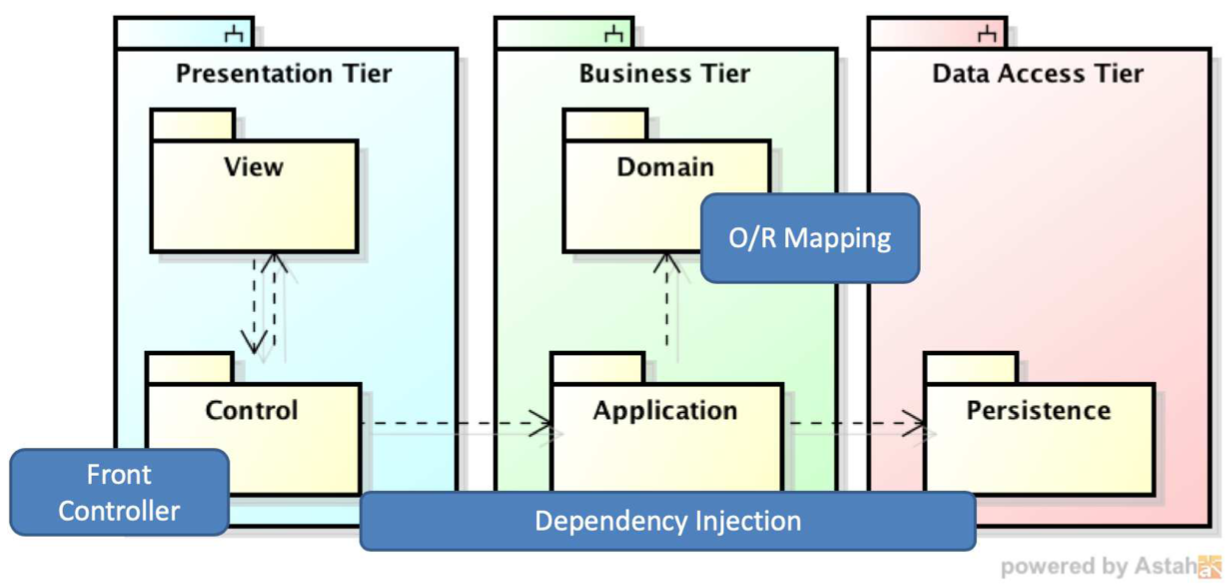
\includegraphics[width=.9\textwidth]{figuras/fig-arquitetura-frameweb.png} 
    \caption{Arquitetura sugerida pelo método FrameWeb~\cite{souza:2020}.}
    \label{fig-arquitetura-frameweb}
\end{figure}


\begin{itemize}
    \item \textbf{Lógica de Apresentação}: tem o objetivo de prover a interface gráfica
        ao usuário e é dividida em dois pacotes. O primeiro é o pacote \textbf{Visão},
        que contém as páginas \textit{Web}, folhas de estilo, imagens, scripts que executam do lado do cliente,
        e outros arquivos relacionados exclusivamente com a exibição de informações ao usuário.
        O segundo é o pacote \textbf{Controle}, que envolve classes de ação que lidam com as requisições
        feitas pelos componentes do pacote \textbf{Visão}, utilizando a infraestrutura do \textit{framework} 
        Controlador Frontal e chamando serviços oferecidos pelo pacote \textbf{Aplicação};

    \item \textbf{Lógica de Negócio}: tem o objetivo de prover os serviços do sistema e é dividida
        em dois pacotes. O primeiro é o pacote \textbf{Aplicação}, que implementa os casos de uso 
        definidos na especificação de requisitos. O segundo é o pacote \textbf{Domínio}, que contém 
        as classes de domínio do sistema, que representam conceitos do domínio do problema;

    \item \textbf{Lógica de Acesso a Dados}: tem o objetivo de prover a persistência dos dados e 
        possui um único pacote, chamado \textbf{Persistência}. Esse pacote é responsável pelo armazenamento
        dos objetos em mídias de longa duração, como bancos de dados. O FrameWeb propõe ainda o uso de um
        \textit{framework} ORM (\textit{Object-Relational Mapping}) com o padrão DAO (\textit{Data Access Object})~\cite{alur:2003}
        para adicionar uma camada de abstração a mais na manipulação de objetos no banco de dados relacional.
\end{itemize}

Além das arquiteturas lógicas e físicas do sistema, é também na fase de Projeto de Sistema
que são modelados os artefatos que serão implementados na próxima etapa. O FrameWeb define
quatro modelos baseados no diagrama de classes UML~\cite{souza:2007,souza:2020}:


\begin{itemize}
    \item \textbf{Modelo de Entidade}: diagrama de classes UML representando o domínio do 
        problema e o mapeamento dos objetos que serão persistidos. Esse modelo tem um forte
        papel para a implementação da Camada de Domínio;

    \item \textbf{Modelo de Persistência}: diagrama de classes UML que representa as classes
        DAO. Para cada uma das classes de domínio que será persistida, é criada uma classe DAO
        que define os métodos de persistência para uma dada classe, guiando assim a 
        construção da Camada de Persistência;
    
    \item \textbf{Modelo de Navegação}: diagrama de classes UML que representa as páginas \textit{Web}
        e outros elementos da Camada de Apresentação. Esse modelo auxilia o desenvolvedor a
        implementar os pacotes Visão e Controle uma vez que todos os atributos e fluxos de 
        navegação baseados nos estímulos enviados pelo usuário são definidos nele;

    \item \textbf{Modelo de Aplicação}: diagrama de classes UML que representa as classes
        responsáveis pela implementação dos casos de uso, além das dependências dos pacotes
        Controle, Domínio e Persistência.
\end{itemize}

A proposta inicial do método FrameWeb foi feita pensando em \textit{frameworks} MVC \cite{souza:2007},
no entanto, com a popularidade dos \textit{frameworks} SPA, o método foi adaptado para suportar
esse tipo de \textit{framework}, que se diferencia do primeiro principalmente pelo fato de possuir elementos que se comportam tanto como \textit{controller} quanto como 
\textit{view} e por focar na interação destes~\cite{hoppe:2023}.


%%%%%%%%% Início de seção. %%%%%%%%%
\section{Frameworks}
\label{sec-fundteo-framework}

\citeonline{schmidt:2004} definem \textit{frameworks} como um conjunto de artefatos de software, sejam eles
classes, objetos ou componentes, que colaboram entre si para prover uma arquitetura reutilizável
para aplicações de uma certa família. Dessa forma, os \textit{frameworks} visam o reuso de soluções, o que
pode reduzir o tempo de desenvolvimento e deixar a manutenção do software mais fácil~\cite{gamma:2000}.

\textit{Frameworks} podem ser classificados de diversas formas, como \textit{frameworks} MVC,
\textit{frameworks} SPA, \textit{frameworks} ORM, entre outros. Nesta seção, serão abordados
com detalhes os \textit{frameworks} ORM e SPA, e por fim, o \textit{framework} utilizado neste trabalho,
que se encaixa nesta categoria.

\subsection{Frameworks SPA}
\label{sec-fundteo-framework-spa}

\textit{Frameworks} SPA (\textit{Single Page Application} ou Aplicações de Página Única) são \textit{frameworks} que implementam
aplicações \textit{Web} executadas por uma única página, ou seja, a página é carregada apenas uma vez 
ao iniciar a aplicação~\cite{emmitt:2015}. Toda a responsabilidade de renderizar a aplicação é
transferida ao \textit{browser} do cliente, o chamado \textit{Client-Side Rendering} (CSR), ou Renderização do Lado do Cliente,
e então o DOM (\textit{Document Object Model} ou Modelo de Documento por Objetos) é manipulado via \textit{JavaScript} para alterar a visualização da 
página~\cite{emmitt:2015,konshin:2018}. Isso faz com que, ao interagir com as páginas, não 
seja necessário carregar a página inteira novamente, apenas os dados e componentes que foram alterados, 
tornando a experiência de usuário mais fluida ao navegar pelo sistema. 

Devido a essa característica, os \textit{frameworks} SPA se tornaram muito populares em aplicações
Web, dentre os mais utilizados estão o Angular\footnote{Angular, \url{https://angular.io}}
e o Vue,\footnote{Vue, \url{https://vuejs.org}} além do React,\footnote{React, \url{https://react.dev}}
que no entanto é uma biblioteca, mas que também implementa aplicações SPA.

No entanto, este tipo de aplicação possui também problemas, sendo eles o alto tempo de carregamento
inicial, pois é necessário carregar todo o código da aplicação de uma vez, e a dificuldade de
indexação por mecanismos de busca (SEO), uma vez que estes tendem a classificar melhor
páginas que carregam mais rápido~\cite{konshin:2018}. Isso é uma grande desvantagem para um sistema
de vendas, por exemplo, que precisa ser indexado por mecanismos de busca para que o site seja mais
fácilmente encontrado por possíveis consumidores.

\subsection{Frameworks ORM}
\label{sec-fundteo-framework-orm}

Grande parte dos sistemas precisam que seus dados sejam armazenados de alguma forma e,
dentre os diversos tipos de sistemas de armazenamento, os bancos de dados relacionais são
os mais utilizados. Esses sistemas possuem uma estrutura de dados organizada em tabelas, e a partir de 
um sistema de gerenciamento de banco de dados relacional (SGBDR), é possível manipular esses dados
por meio da linguagem SQL (\textit{Structured Query Language} ou Linguagem Estruturada de Consulta)~\cite{silberschatz:2019}.

Por outro lado, muitas aplicações utilizam linguagens de programação orientadas a objetos (OO), o que
pode tornar a manipulação de dados em um banco de dados relacional mais complexa, uma vez que
as SGBDR representam os dados como tabelas, enquanto as linguagens OO os representam como um grafo 
de objetos interconectados. Essa é a chamada incompatibilidade de paradigmas (\textit{paradigm mismatch})~\cite{hibernate:2010,bauer:2005}.

Na década de 80, surgiram os \textit{frameworks} ORM (Mapeamento Objeto/Relacional), que têm como objetivo
mapear os objetos da aplicação para as tabelas do banco de dados relacional. O uso desses \textit{frameworks} 
facilita a manipulação de dados para o desenvolvedor, que precisa apenas informar ao \textit{framework}
como transformar objetos e seus atributos em tabelas e colunas e chamar métodos simples, sem precisar
aprender uma nova linguagem como SQL.

Alguns exemplos de \textit{frameworks} ORM são o Hibernate para Java,\footnote{Hibernate, \url{https://hibernate.org}}
Entity Framework para .NET,\footnote{Entity Framework, \url{https://docs.microsoft.com/pt-br/ef}} e o 
Prisma para TypeScript.\footnote{Prisma, \url{https://www.prisma.io}}



\subsection{Next.js}
\label{sec-fundteo-framework-next}


O Next.js é um \textit{framework Web} construído em cima do React, biblioteca JavaScript \textit{front-end open-source}
baseada em componentes, voltada para a construção da interface de usuário e mantida pela Meta.\footnote{Meta, \url{https://about.meta.com}}
Por ser uma biblioteca, o React não implementa 
técnicas de roteamento, o que faz com que exista a dependência do uso de outras bibliotecas, 
como o React Router.\footnote{React Router, \url{https://reactrouter.com}}
Já o Next.js faz isso de forma nativa. 

Outro ponto de destaque são as técnicas de renderização, 
além do CSR, o Next.js implementa os métodos \textit{Server-Side Rendering} (SSR), ou Renderização do Lado do Servidor,
e \textit{Static Site Generation} (SSG), ou Geração Estática de Site, que permitem que o código da aplicação seja executado
no servidor, e resolvem os problemas de SEO e tempo de carregamento inicial, comuns de 
aplicações SPA. Um detalhe que tem feito com que esse \textit{framework}
ganhe popularidade, é o fato de que o desenvolvedor pode escolher qual método de renderização
utilizar para cada página do sistema~\cite{vercel:2023}.

Outro ponto alto do Next.js é a facilidade de se fazer o \textit{deploy} da aplicação, que pode ser feito
de forma otimizada com o provedor de \textit{hosting} da Vercel,\footnote{Vercel, \url{https://vercel.com}} 
plataforma que desenvolveu o \textit{framework}~\cite{nextjs:2023}.

\textit{JavaScript} é uma linguagem leve e interpretada, que é utilizada para adicionar interatividade e dinamicidade
à páginas \textit{Web}. No entanto, por ser uma linguagem de tipagem fraca e dinâmica, ela pode ser propensa a erros
em tempo de execução, o que, em sistemas de porte elevado, pode se tornar um grande problema~\cite{typescript:2024}.
Nesse ambiente, surge o \textit{TypeScript}, linguagem de programação de alto nível desenvolvida e mantida pela Microsoft.\footnote{Microsoft, \url{https://www.microsoft.com}}
O \textit{TypeScript} é convertido em código \textit{JavaScript}, e portanto fornece todas as características desta, além de adicionar suporte a tipos, 
permitindo a detecção de erros em tempo de compilação,
e outras funcionalidades, como interfaces, \textit{generics} e \textit{unions}~\cite{typescript:2024}.

O Next.js suporta o uso de \textit{TypeScript} em suas aplicações, o que pode ser uma grande vantagem para
desenvolvedores que desejam ter um código mais seguro e menos propenso a erros.

% \vitor{Esta seção está muito pequena. Se você está falando de TypeScript por ela ser a linguagem usada no desenvolvimento com Next.js, então você pode incluir essa informação e mais este parágrafo na seção do Next.js.}
